\section{Oracle-based scheme for the detection of faults}\label{sec:faultDetection}
In ~\ref{sec:prediction}, we described a way to systematically predict when a fault is not critical (i.e. does not prevent the execution from converging) by looking at its symptoms on the execution variables. In this section, we will use this result to propose and evaluate a fault detection scheme. In~\ref{sec:detection_oracle}, the method is described and each outcome is illustrated, and is evaluated extensively in~\ref{sec:evaluation_oracle}

\subsection{Description of the detection scheme} \label{sec:detection_oracle}
From the ability to systematically predict if a fault is non-critical, a fault detection scheme can easily be derived by ignoring faults that we are sure will not disrupt the convergence, and by triggering the detection otherwise. 

Let $0 < c < 1 $. This detection scheme would be as follow:
\begin{enumerate}
\item Set the target accuracy to $(1-c) \cdot \varepsilon$.
\item At the fault iteration $f$, perform the following test:

\begin{equation} 
	error =  \|{w}_{f+1} - \widetilde{w}_{f+1}\| < \tau_c = c \cdot \varepsilon / |y_{\ell, f}|
\end{equation}\label{detection_scheme_oracle}
\item If the error is smaller than the threshold, the fault is ignored as it does not threaten the convergence, otherwise, a detection is triggered. 
\end{enumerate}


Table \ref{table:theoretical_outcomes} gathers the 4 possible outcomes produced by this detection scheme. If the execution converges, the fault is said to have no impact, whereas a fault preventing the execution from converging is said to be critical. 

\begin{table}[h]
\centering
\caption{Colors and name used for each test outcome.}
\label{table:theoretical_outcomes}
\begin{tabular}{l|ll|}
	& Convergence & No convergence\\
    \hline
   Detection & \color[RGB]{30, 30, 30}{\textbf{No impact fault detected}} & \color[RGB]{85, 147, 47}{\textbf{Critical fault detected}} \\
 
   No detection & \color[RGB]{90, 90, 90}{\textbf{No impact fault ignored}} & \color{red}{\textbf{Critical fault ignored}} \\
    \hline
\end{tabular}
\end{table}

Figure \ref{fig:conv_hist_detection_correct} plots 2 convergence histories for each algorithm. In figures \ref{fig:gre_216a_conv_hist_theoretical_detection_0} and 
\ref{fig:pores_2_conv_hist_theoretical_detection_0}, no fault is detected as the error is smaller than the threshold, and the executions converges, producing a \emph{No impact fault ignored} from Table~\ref{table:theoretical_outcomes}. In figures \ref{fig:gre_216a_conv_hist_theoretical_detection_1} and 
\ref{fig:pores_2_conv_hist_theoretical_detection_1}, a critical fault is detected as the error is greater than the threshold $\tau_{0.5}$ at the fault iteration and the executions does not converge, producing a \emph{Critical fault detected} from Table~\ref{table:theoretical_outcomes}. In both cases, the fault is properly detected.






\begin{figure}[h]
	\centering
    
\begin{minipage}[b]{0.45\linewidth}
\centering
\textbf{GMRES} executions on \textbf{gre_216a} 
\end{minipage}
\quad
\begin{minipage}{0.45\linewidth}
\centering
\textbf{preconditioned-GMRES} on \textbf{pores_2}
\end{minipage}\\


    \begin{minipage}[b]{0.48\linewidth}
	
	\begin{subfigure}[t]{\linewidth}
		\centering
		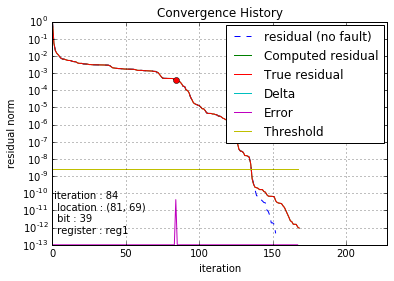
\includegraphics[width=\linewidth]{figures/gre_216a/convergence_history_theoretical_detection_1_1.png}
		\caption{No impact fault ignored}\label{fig:gre_216a_conv_hist_theoretical_detection_0}
	\end{subfigure}
    \quad
    \begin{subfigure}[t]{\linewidth}
		\centering
		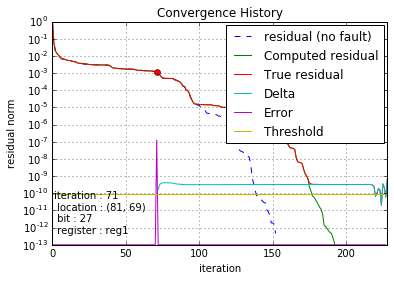
\includegraphics[width=\linewidth]{figures/gre_216a/convergence_history_theoretical_detection_0_1.png}
		\caption{Critical fault detected}\label{fig:gre_216a_conv_hist_theoretical_detection_1}
	\end{subfigure}
    \end{minipage}
    \quad
    \begin{minipage}[b]{0.48\linewidth}
    	
	\begin{subfigure}[t]{\linewidth}
		\centering
		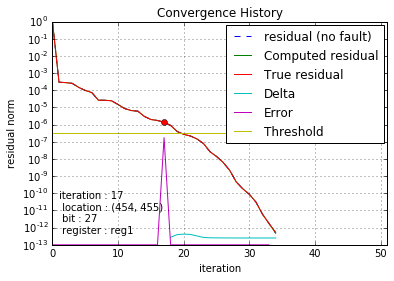
\includegraphics[width=\linewidth]{figures/pores_2/convergence_history_theoretical_detection_1_1.png}
		\caption{No impact fault ignored}\label{fig:pores_2_conv_hist_theoretical_detection_0}
	\end{subfigure}
    \quad
    \begin{subfigure}[t]{\linewidth}
		\centering
		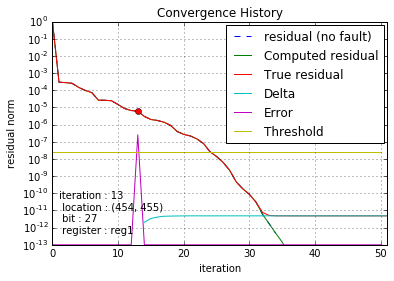
\includegraphics[width=\linewidth]{figures/pores_2/convergence_history_theoretical_detection_0_1.png}
		\caption{Critical fault detected}\label{fig:pores_2_conv_hist_theoretical_detection_1}
	\end{subfigure}

    
	\end{minipage}
\caption{Convergence histories of 2 GMRES executions on HB/gre_216a and 2 preconditioned-GMRES executions on HB/pored_2, disrupted by transient faults that are properly detected. The error and the threshold are plotted. In figures~\ref{fig:gre_216a_conv_hist_theoretical_detection_0} and~\ref{fig:pores_2_conv_hist_theoretical_detection_0}, the error at each iteration remains below the threshold, so no fault is detected and the execution converges, producing a \emph{No impact fault ignored} from Table \ref{colors}. In figures~\ref{fig:gre_216a_conv_hist_theoretical_detection_1} and~\ref{fig:pores_2_conv_hist_theoretical_detection_1}, the error becomes higher than the threshold at the fault iteration, so the fault is detected and the execution does not converge, producing a \emph{Critical fault detected} from Table \ref{table:theoretical_outcomes}. }\label{fig:conv_hist_detection_correct}
\end{figure}



\subsection{Evaluation of the detection scheme}\label{sec:evaluation_oracle}
The remaining parameter to be chosen is $c$. One intuitive way to understand this parameter's role is as follow: in order to control the accuracy of the true residual norm, we split it into two quantities easier to control. On the one hand, the computed residual norm can be adjusted by setting the target accuracy of the execution to the desired value, at the expense of additional computation, and on the other hand the residual gap can be measured and allowed to grow before triggering a detection. However those two values cannot be adjusted independently to ensure the true residual norm convergence to the target accuracy, so the $c$ parameter aims at balancing the importance of one or the other value (computed residual or residual gap). So if one wishes to decrease the sensitivity of the detection scheme, he should increase the $c$ value to allow the residual gap to grow larger before triggering a detection, at the expense of more iterations to reduce the computed residual norm. On the contrary if one does not want to use too much additional iterations to reduce the computed residual norm, he gets a more sensitive detection scheme that is efficient for detecting critical faults, but may also detect faults that do not have any impact on the convergence.


In the following, numerical experiments are performed to evaluate the detection scheme quality. Figure~\ref{fig:test_result_oracle} displays the fault detection scheme results (in percentage of executions) for several values of c.
First, no critical faults are ignored, which is a direct consequence of Theorem \ref{theorem}: if a fault is ignored (the error is smaller than the threshold), then the execution must converge. Second, for low values of $c$, an important part (between 20\% and 35\%) of executions disrupted by a negligible fault detect it anyway (dark gray) as the detection scheme is more sensitive, but it becomes more and more capable of ignoring those when $c$ increases. The rest of the faulty executions (green and light gray) are correctly handled.

For more details, the $c=0.5$ cases are plotted in Figure~\ref{fig:test_result_c05}. In each case, a large majority of the faulty executions correctly detects the faults. The rare cases of unneeded detection (dark gray) occur at the limit of the convergence and non convergence domain (light gray and green respectively).

Overall, the detection quality is very good as all critical faults have been properly detected, and only a few negligible faults were unnecessarily detected. Indeed, even though we do not have the reverse of Theorem~\ref{theorem} (which would ensure that \emph{only} executions in which faults are ignored by the detection scheme does converge, hence removing the dark gray outcomes), this numerical experiment shows that the reverse is not far from being true.






\begin{figure}[h]
	\centering
    
\begin{minipage}[b]{0.45\linewidth}
\centering
\textbf{GMRES} executions on \textbf{gre_216a} 
\end{minipage}
\quad
\begin{minipage}{0.45\linewidth}
\centering
\textbf{preconditioned-GMRES} on \textbf{pores_2}
\end{minipage}\\


    \begin{minipage}[b]{0.48\linewidth}
	
	\begin{subfigure}[t]{\linewidth}
		\centering
		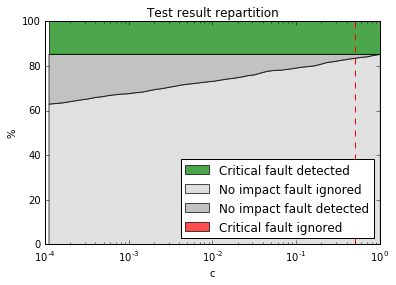
\includegraphics[width=1.1\linewidth]{figures/gre_216a/test_result_oracle_0.png}
		\caption{$\varepsilon = 10^{-6}$}\label{fig:gre_216a_test_result_oracle_0}	
	\end{subfigure}
    \quad
    \begin{subfigure}[t]{\linewidth}
		\centering
		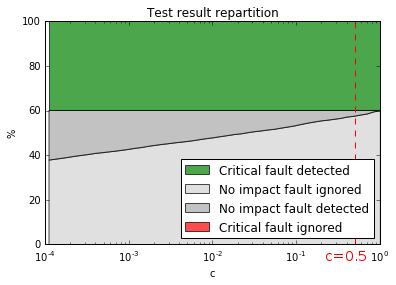
\includegraphics[width=1.1\linewidth]{figures/gre_216a/test_result_oracle_1.png}
		\caption{$\varepsilon = 10^{-12}$}\label{fig:gre_216a_test_result_oracle_1}	
	\end{subfigure}
    \end{minipage}
    \quad
    \begin{minipage}[b]{0.48\linewidth}
    	
	\begin{subfigure}[t]{\linewidth}
		\centering
		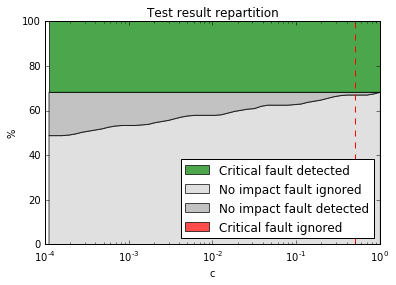
\includegraphics[width=1.1\linewidth]{figures/pores_2/test_result_oracle_0.png}
		\caption{$\varepsilon = 10^{-6}$}\label{fig:pores_2_test_result_oracle_0}	
	\end{subfigure}
    \quad
    \begin{subfigure}[t]{\linewidth}
		\centering
		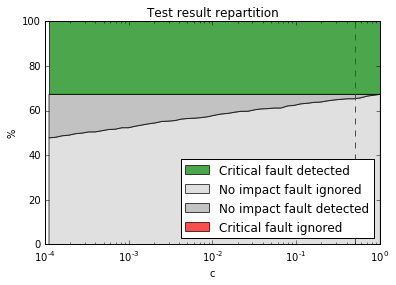
\includegraphics[width=1.1\linewidth]{figures/pores_2/test_result_oracle_1.png}
		\caption{$\varepsilon = 10^{-12}$}\label{fig:pores_2_test_result_oracle_1}	
	\end{subfigure}

	\end{minipage}
\caption{Diagrams representing the test outcome proportion for several values of c. To compute them, faulty executions covering a large part of the fault parameter space were performed. The case $c = 0.5$ represented by the dashed red line is detailed in Figure~\ref{fig:test_result_oracle_c05}.}\label{fig:test_result_oracle}
\end{figure}




\begin{figure}[h]
	\centering
    
\begin{minipage}[b]{0.45\linewidth}
\centering
\textbf{GMRES} executions on \textbf{gre_216a} 
\end{minipage}
\quad
\begin{minipage}{0.45\linewidth}
\centering
\textbf{preconditioned-GMRES} on \textbf{pores_2}
\end{minipage}\\


    \begin{minipage}[b]{0.48\linewidth}
	
	\begin{subfigure}[t]{\linewidth}
		\centering
		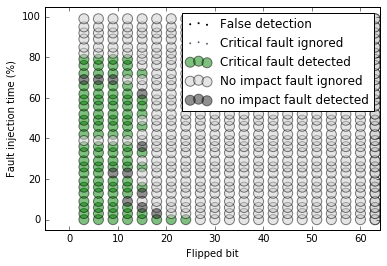
\includegraphics[width=1.1\linewidth]{figures/gre_216a/test_result_c05_oracle_0.png}
		\caption{$\varepsilon = 10^{-6}$}\label{fig:gre_216a_test_result_c05_oracle_0}	
	\end{subfigure}
    \quad
    \begin{subfigure}[t]{\linewidth}
		\centering
		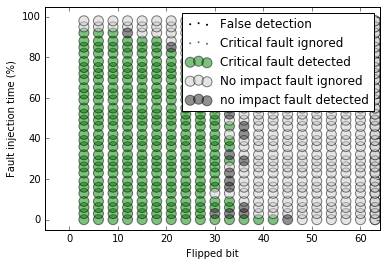
\includegraphics[width=1.1\linewidth]{figures/gre_216a/test_result_c05_oracle_1.png}
		\caption{$\varepsilon = 10^{-12}$}\label{fig:gre_216a_test_result_c05_oracle_1}	
	\end{subfigure}
    \end{minipage}
    \quad
    \begin{minipage}[b]{0.48\linewidth}
    	
	\begin{subfigure}[t]{\linewidth}
		\centering
		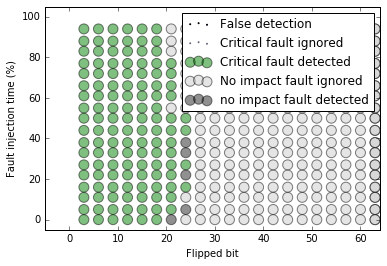
\includegraphics[width=1.1\linewidth]{figures/pores_2/test_result_c05_oracle_0.png}
		\caption{$\varepsilon = 10^{-6}$}\label{fig:pores_2_test_result_c05_oracle_0}	
	\end{subfigure}
    \quad
    \begin{subfigure}[t]{\linewidth}
		\centering
		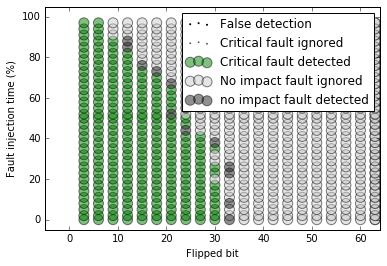
\includegraphics[width=1.1\linewidth]{figures/pores_2/test_result_c05_oracle_1.png}
		\caption{$\varepsilon = 10^{-12}$}\label{fig:pores_2_test_result_c05_oracle_1}	
	\end{subfigure}

	\end{minipage}
\caption{Diagram detailing the test results for $c = 0.5$. Each dot corresponds to a faulty execution, and its color represents the test outcome from Table \ref{table:theoretical_outcomes}.}
\label{fig:test_result_oracle_c05}
\end{figure}










